\begin{table}
  \footnotesize
  \centering
  \begin{tabular}{c c c c}
    \toprule
    Application & Knobs & Utility & Dataset \\
    \midrule
    \specialcell{Pedestrian\\Detection}
                & \specialcell{resolution \\ frame rate \\ quantizer }
                & F1 score & \specialcell{MOT16~\cite{milan2016mot16}\\training: MOT16-04\\testing: MOT16-03} \\
    \midrule
    \specialcell{Augmented\\Reality}
                & \specialcell{resolution \\ frame rate \\ quantizer }
                & F1 score & \specialcell{iPhone video clips\\training: office (24 s)\\testing: home
    (246 s)} \\
    \midrule
    \specialcell{Log Analysis\\(Top-K)}
                & \specialcell{head (N) \\ threshold (T) }
                & \specialcell{Kendall's $\tau$}
                        & \specialcell{\href{https://www.sec.gov}{SEC.gov} access logs~\cite{edgarlog} \\ training: 4 days \\
    testing: 16 days} \\
    \bottomrule
  \end{tabular}
  \caption{\sysname{} Applications}
  \label{tab:apps}
\end{table}

\section{Implementation and Applications}
\label{sec:implementation}

While our proposed APIs are general and not language specific, we choose a safe
language, Rust, to implement the core framework. \sysname{} is open-source on
Github.\footnote{Url elided for anonymity.} Applications built with \sysname{}
run as a single process. The entire processing pipeline is often specified in a
single main file. The execution mode (profiling, runtime as client or runtime as
server) is configured with command line arguments or environment variables. Our
deployment manager is currently a shell script.

% First, Rust's memory safety guarantee can ensure applications running
% continously for an extended period of time. Besides, the zero-cost abstraction
% removes the possibilities of tail latencies caused by uncoordinated garbage
% collection~\cite{maas2016taurus}. In addition, we rely on Rust's type system
% to enforce the type match on \texttt{maybe} operations.

% All operators implement the \texttt{Stream} trait which has an associate type
% \texttt{Item} and a core function \texttt{next} that returns
% \texttt{Datum}. Each datum is either an item with the \texttt{Stream::Item} or
% an \texttt{Error} that the operator use to communicate with the runtime
% scheduler. The concrete form of \texttt{maybe} API is almost an direct
% translation of the API specification. While our API specification
% in~\autoref{tab:operators} uses a vector for knobs, our Rust implementation is
% more general: any type (including vector) that implements \texttt{IntoKnob}
% trait can be used as the knob.
% \begin{lstlisting}
% pub trait Stream {
%     type Item;
%     fn next(&mut self) -> Datum<Self::Item, Error>;

%     fn maybe<K, F>(self, opts: K, f: F) -> Maybe<Self, F>
%         where Self: Sized,
%                 K: IntoKnob,
%                 F: FnMut(K::Item, Self::Item) -> Self::Item {

%          // omitted
%     }
% }
% \end{lstlisting}

% \begin{figure*}
%   \centering
%   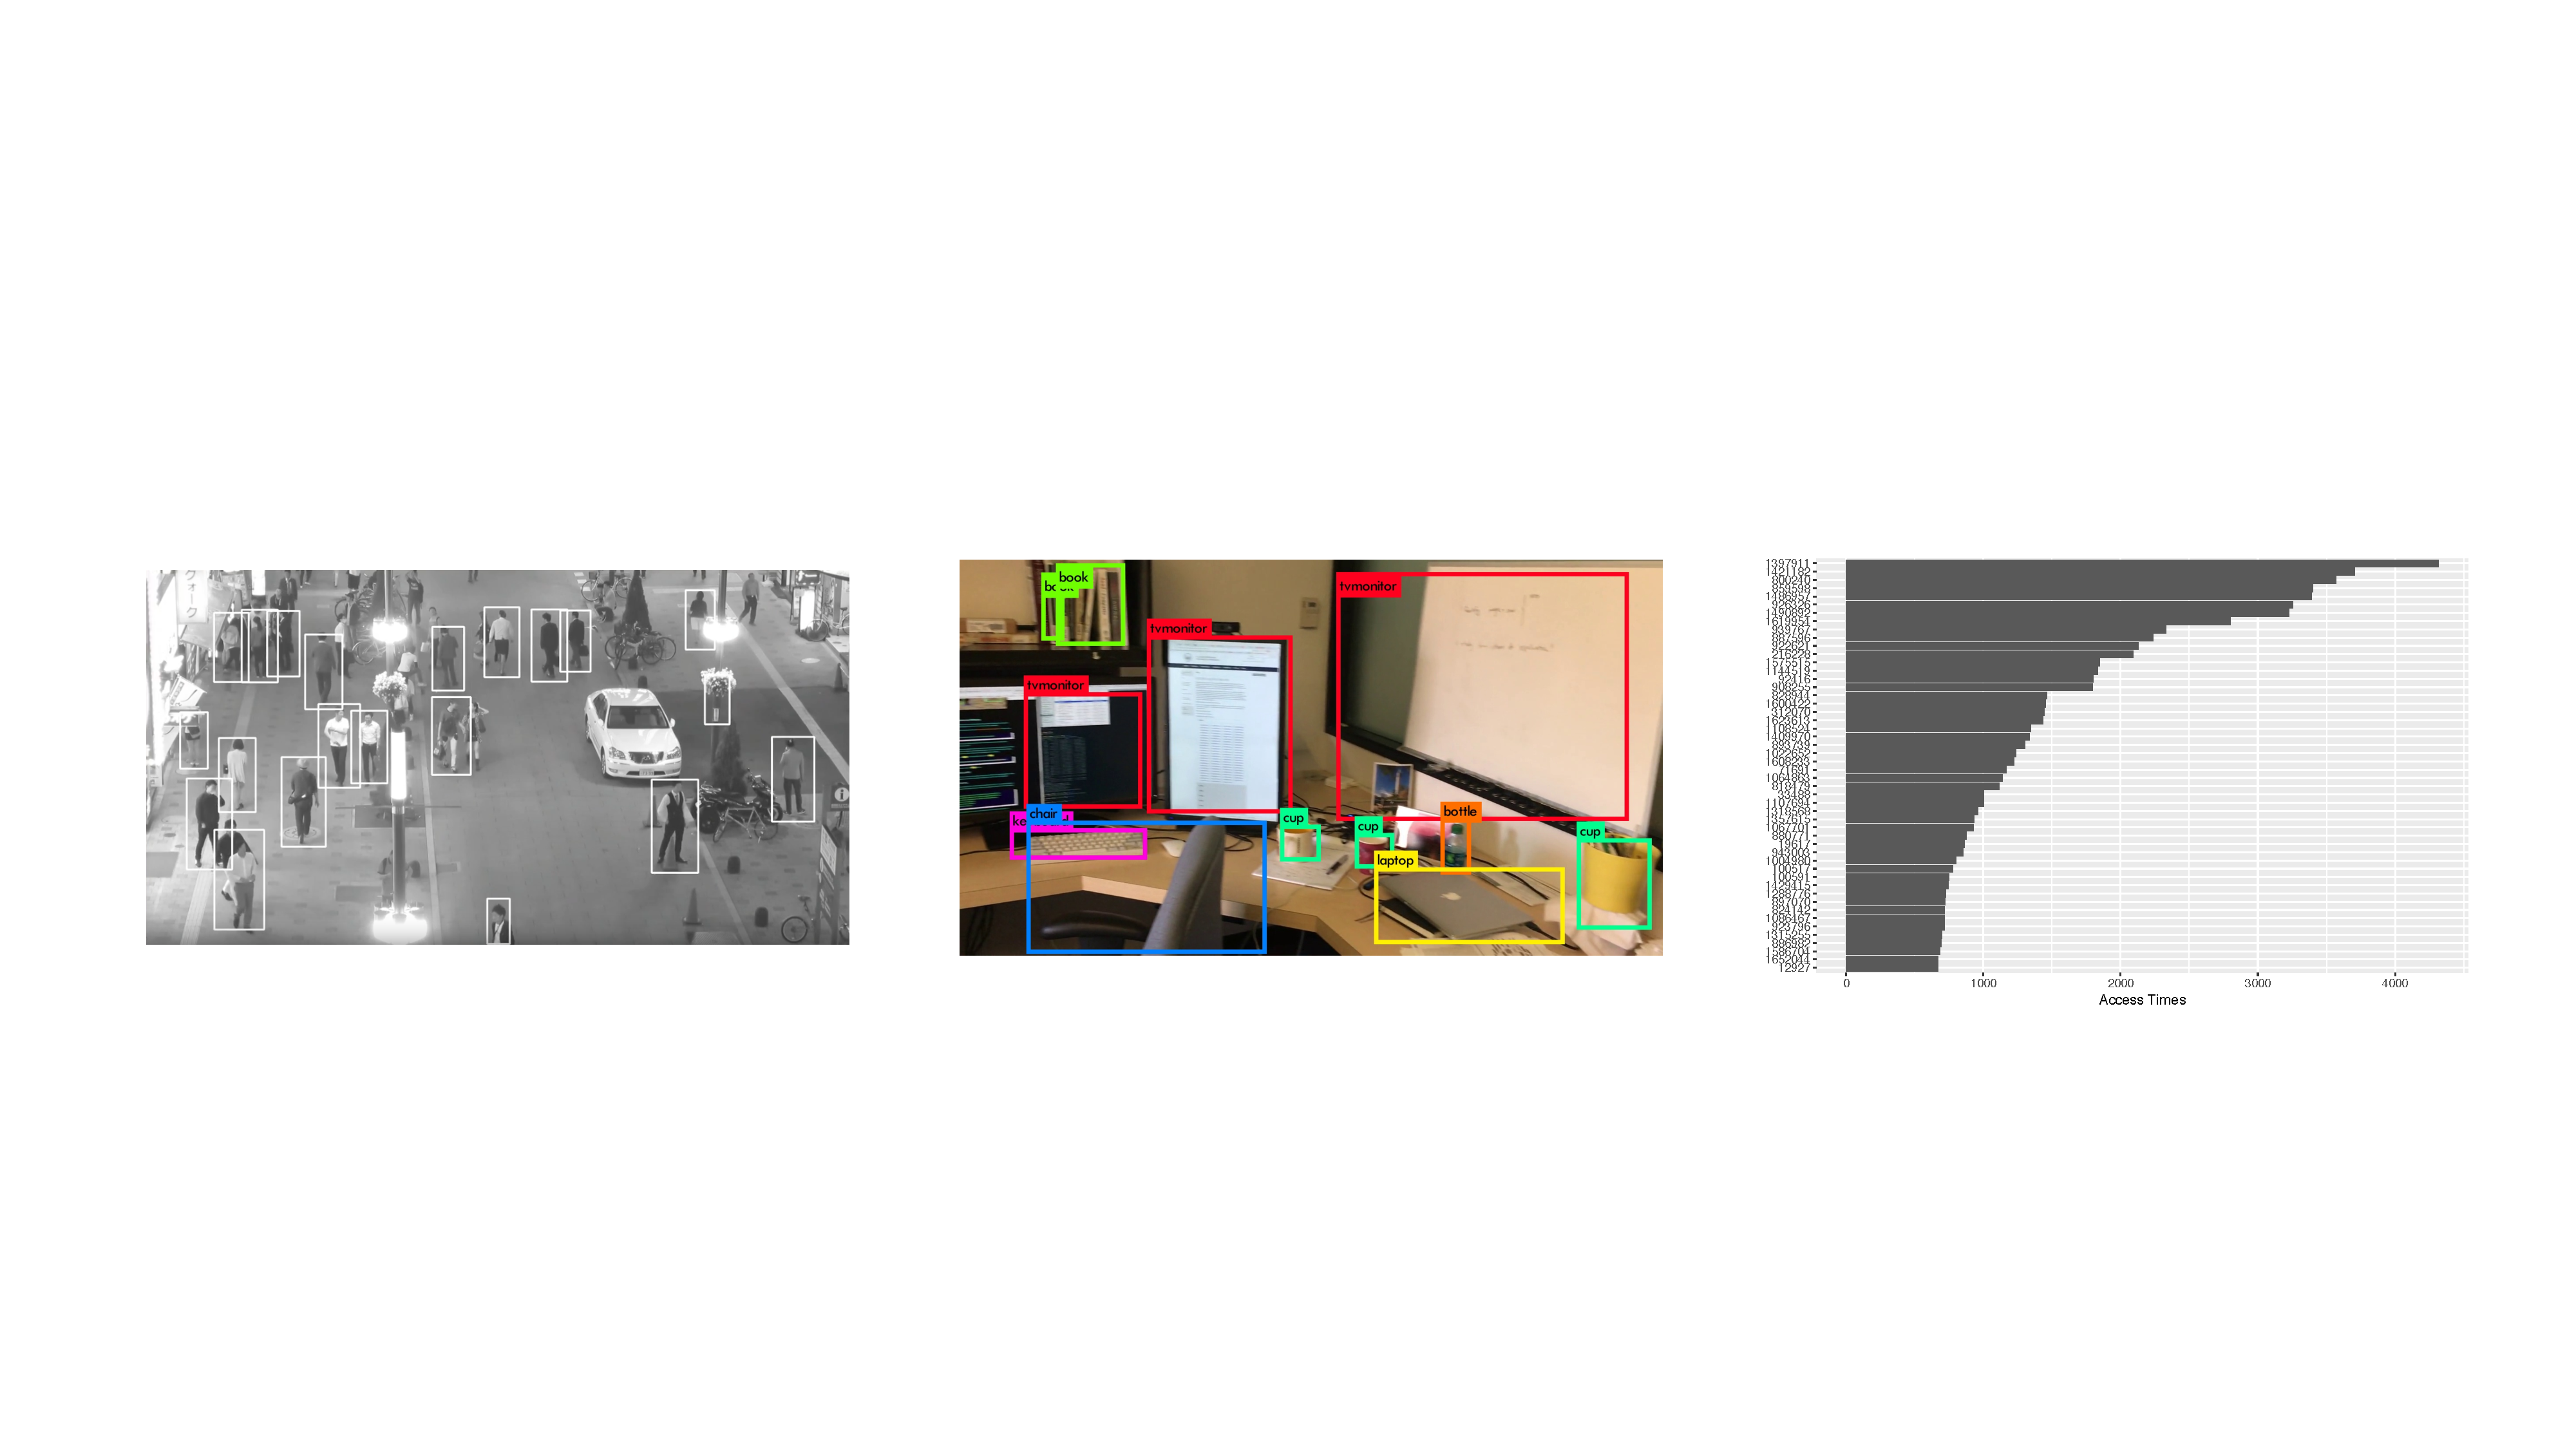
\includegraphics[width=\textwidth]{figures/apps.pdf}
%   \caption{Applications}
%   \label{fig:apps}
% \end{figure*}

We've built built three applications: pedestrian detection surveillance, an
augmented reality, and a distributed log analysis to extract the Top-K most
access files. \autoref{tab:apps} summarizes the application-specific part:
knobs, utility function, and the dataset we used for training and testing.

\para{Pedestrian Detection:} This application analyzes streams of videos from
installed CCTV cameras and detects pedestrians inside. We implement
image-related operations with OpenCV 3.1~\cite{opencvlibrary} and detect
pedestrians with histogram of oriented gradients
(HOG)~\cite{dalal2005histograms} with the default linear SVM classifier. To
ensure real-time processing of frames, we use the GPU-accelerated
implementation. Video encoding employs H.264 scheme because of its prevalence in
existing systems. Our implemenation is based on GStreamer~\cite{gstreamer} with
\texttt{x264enc} plugin. To integrate with \sysname{}, we first create a
pipeline that exposes \texttt{appsrc} (to feed raw image data) and
\texttt{appsink} (to get encoded bytes). The GStreamer main loop is managed in a
separate thread and \sysname{} communicates with it via Rust's channel. The
\texttt{x264enc} is configured with \texttt{zerolatency} preset and uses four
threads. We use constant quality encoding and expose the quantizer as another
knob.

Pedestrian detection returns a list of bounding boxes, and each box is a
rectangle with normalized coordinates on the image. The detection is compared
against the reference result from raw data. A detection is successful if the
intersection over union (IOU) is greater than
50\%~\cite{everingham2010pascal}. We use F1 score
(\%)~\cite{Rijsbergen:1979:IR:539927} as the accuracy function and MOT16
dataset~\cite{milan2016mot16} for training and testing.

\para{Augmented Reality:} We target at mobile augmented reality applications
that recognizes objects by offloading the heavy computation to resources
elsewhere. Even when the offloading server is
nearby~\cite{satyanarayanan2009case, zhang2015cloud}, the wireless communication
link is still susceptible to capacity variation.

We use a similar setup (OpenCV and GStreamer) as the pedestrian detection except
for the actual analytical function. To recognize objects, we use
YOLO~\cite{darknet13, redmon2016yolo9000}, a GPU-enabled pre-trained system for
object detection. In this case, a successful detection requires matching the
object type in addition to IOU criteria.

\para{Distributed Top-K:} Many monitoring applications need to answer the
\textit{Top-K} question~\cite{babcock2003distributed}, such as the Top-K most
popular URLs, or the Top-K most access files. A distributed Top-K application
aggregates information from geo-distributed servers (see \autoref{fig:topk} for
an illustration).

\begin{figure}
  \centering
  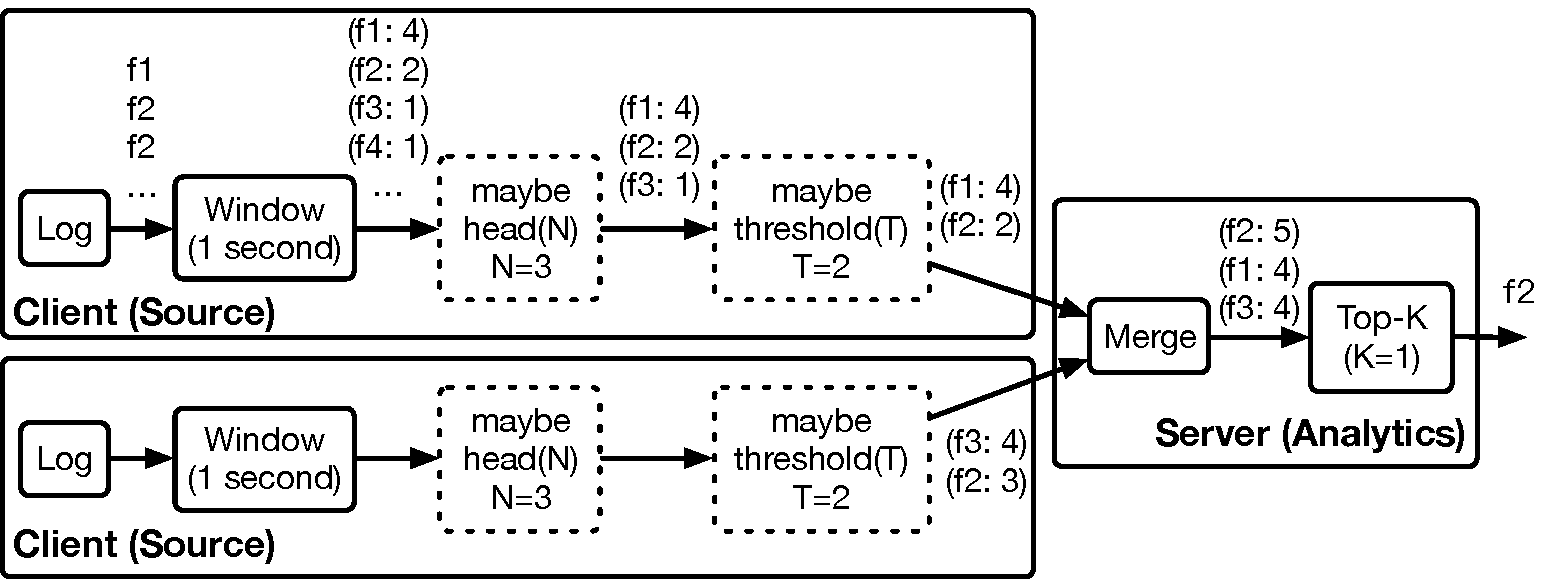
\includegraphics[width=\columnwidth]{figures/topk.pdf}
  \caption{A distributed Top-K application with two degradation operations:
    \texttt{head} and \texttt{threshold}.}
  \label{fig:topk}
\end{figure}

Naively aggregating all the raw logs is not feasible because popular servers
have millions of requests per second. Edge nodes can first perform a
\texttt{Window} operation to generate data summary, such as key-value pairs of
\texttt{<item, count>}. However, even after this operation, the data size can
still be too large because most real-world access patterns follow a long-tailed
distribution. There is a large-but-irrelevant tail that contributes little to
the final results.

The edge nodes perform two degradation operations: (1) a head (\texttt{N})
operation that only takes the top \texttt{N} entries; (2) a threshold \texttt{T}
that filters small entries. These two operations are not orthognal to each
other. Their impact on data size reduction and quality degradation depends on
the distribution of the actual data. The accuracy function is
Kendall's~$\tau$~\cite{abdi2007kendall}. It is a correlation measure of the
concordance between two ranked list. The output ranges from -1 to 1,
representing no agreement to complete agreement, respectively. To integrate with
\sysname{}, we convert the measure with a linear transformation to the range of
[0, 1].

Our Top-K application aims to find the fifty most accessed files from web server
logs. We use Apache logs files that record and store user access statistics for
the \href{https://www.sec.gov}{SEC.gov} website. These log files are split into
four groups, simulating four geo-distributed nodes. We also compress an hour's
logs into one second to match the load of popular web servers.

%%% Local Variables:
%%% mode: latex
%%% TeX-master: "sosp17"
%%% End:
